\documentclass[twoside,11pt]{cergdoc}
\usepackage{graphicx}
\usepackage{amsmath}

\begin{document}

\title{XXBX Power Shim -- XBP}
\subtitle{XBP User Guide v1.0}
\author{Jens-Peter Kaps}
\email{jkaps@gmu.edu}
\affiliation{George Mason University\\
  Fairfax, Virginia}
\topicpic{xxbx-slide}

\maketitle

\tableofcontents

% -----------------------------------------------------------------------------
\chapter{Introduction}
% -----------------------------------------------------------------------------
The XXBX Power Shim (XBP) connects the Harness (XBH) to the Device under test (XBD). Figure~\ref{fig:xxbxsetup}
shows a typical XXBX setup with the XBP placed between the XBH and the XBD. All signals from the 
XBH to the XBD pass through the XBP. The main purpose of the XBP is to sense the current 
drawn by the XBD, amplify its value and pass it on to the XBH for measurement. 

\begin{figure}[ht]
  \begin{center}
    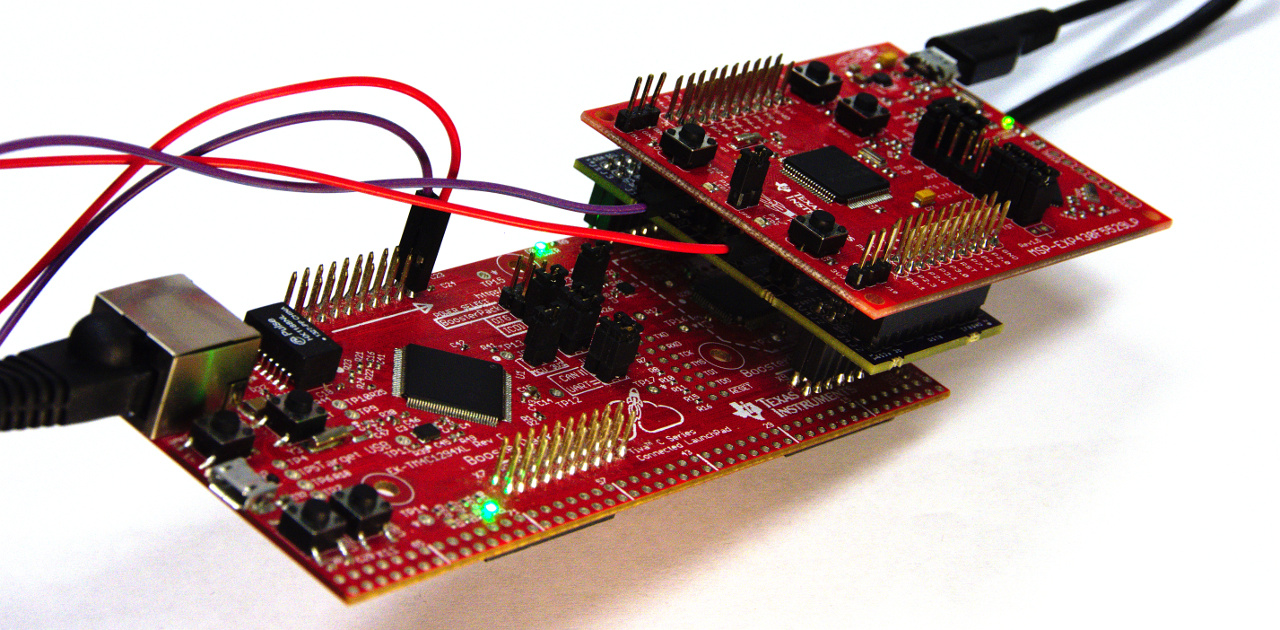
\includegraphics[scale=1]{figures/xxbx-setup-side}
    \caption{XXBX Setup with XBH on the bottom followed by XBP in the middle and XBD on top}\label{fig:xxbxsetup}
  \end{center}
\end{figure}

\section{XBP Current Sensing and Amplification}\label{sec:sensing}
The power consumed by a device can be computed from the current $I$ that it draws and
its supply voltage $\mathrm{V_{CC}D}$ as $P = I \cdot V_{CC}D$. The energy it 
consumes for executing a particular task is the integral of $P$ over the run time.
As the voltage $V_{CC}D$ is fixed for a particular XBD we only have to measure 
the current.

The current is measured by sensing the voltage drop across a small shunt resistor $R_S$.
The shunt resistor could be placed between the voltage source and the device
or between the device and ground called high-side and low-side current sensing
respectively. We opted for high-side current sensing (see Fig\,\ref{fig:block})
as it eliminates the problems associated with multiple ground paths. 
The drawback of high-side sensing is the higher common-mode voltage which is the
average voltage before and after the shunt. 


The shunt resistor should be very small as to not have a large influence on 
the supply voltage of the XBD, however that means that voltage drop across the shunt will
also be very small. Therefore, it has to be amplified before it can be measured by 
an analog to digital converter (ADC). Furthermore, the low input resistance
of ADCs makes a direct measurement unfeasible.  
Hence, we use a current-shunt monitor (CSM), i.e.\ the INA225 from Texas Instruments.
It has a programmable gain setting between 25 and 200, a buffered output so that it
can drive an ADC input, a bandwidth of 125\,kHz, and supports high common-mode voltages.

The formula for the resolution of the ADC is shown in~\eqref{eq:adcres}. The maximum input voltage
to the ADC ($V_{CSMmax}$) is 3.3V and its resolution is 12\,bits. 
\begin{equation}
  V_{res}=\frac{V_{CSMmax}}{2^{ADCbits}} = \frac{3.3\,\mathrm{V}}{2^{12}\,\mathrm{bits}} = 0.8\,\mathrm{mV} \label{eq:adcres}
\end{equation}

The voltage applied to the ADC depends on the voltage drop $V_S$ across the shunt resistor
$R_S$ and the gain of the CSM $\delta_{CSM}$. This relationship is expressed in~\eqref{eq:csm}.
\begin{equation}
  V_{CSM} = V_S \cdot \delta_{CSM} = R_S \cdot I \cdot \delta_{CSM} \label{eq:csm}
\end{equation}

When using a 1\,$\Omega$ resistor for $R_S$ we achieve for a gain factor of 25 a resolution of
%
\[I_{res} = \frac{V_{res}}{R_S \cdot \delta_{CSM}} = \frac{0.8\,\mathrm{mV}}{1\,\Omega \cdot 25} = 32\,\mathrm{\mu A}\]
%
and can measure a current of at most
%
\[I_{max} = \frac{V_{CSMmax}}{R_S \cdot \delta_{CSM}} = \frac{3.3\,\mathrm{V}}{1\,\Omega \cdot 25} = 132\,\mathrm{mA}.\]
%
%a current resolution of 16.5\,$\mu$A at 200 gain, topping out at 32\,mA, 
%and 132\,$\mu$A resolution at a gain of 25 topping out at 132\,mA.
%
At the maximum gain of 200 the resolution is $4.0\,\mathrm{\mu A}$ and the maximum current is 16.5\,mA.


\begin{figure}[ht]
  \begin{center}
    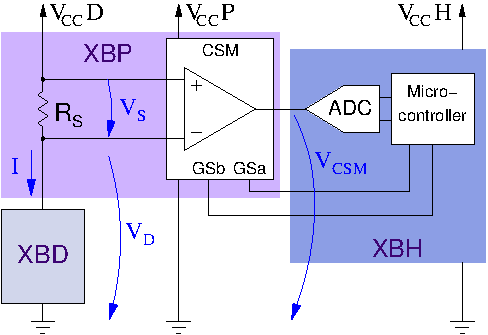
\includegraphics[scale=1]{figures/ina225}
    \caption{Block Diagram of the Power Measurement Setup}\label{fig:block}
  \end{center}
\end{figure}

\section{Voltage Level Shifter}\label{sec:shifter}
Some XBDs might require a supply voltage $V_{CC}D$ which is higher than the $V_{CC}H = 3.3$\,V
or lower. As all control signals for the XBD pass through the XBP, we added circuitry for
voltage level shifting. The circuit used on the XBP is shown in Fig\,~\ref{fig:voltagelevel}. 

When SDA is not active or any side wants to transmit a logic `one', the pull-up resistors on both 
sides pull the inputs on the XBD and the XBH to their voltage levels. 
When the XBH pulls down SCL, the source input of the transistor Q6 becomes low, while the gate stays high. 
$V_{GS}$ rises above the threshold and the transistor conducts. This pulls down the 
the drain input of Q5. Now the drain-substrate diode of Q5 is pulled down until $V_GS$ passes the
threshold and the transistor conducts, hence
SDA on the XBD is low. 
Due to symmetry, XBD can pull down SDA in a similar fashion which results in SDA on XBH going low.
While single transistor solutions exist that can accomplish the same functionality,
only this 2 transistor circuit is agnostic to whether the XBD side or the XBH side has a higher
$V_CC$, i.e.\ it allows the use XBDs with higher as well as with lower supply
voltages. 

\begin{figure}[ht]
  \begin{center}
    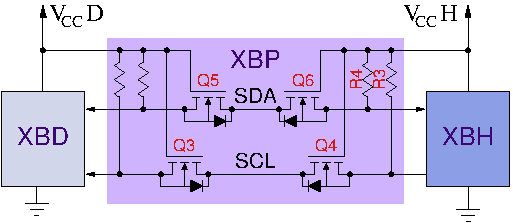
\includegraphics[scale=1]{figures/voltagelevel}
    \caption{Voltage Level Shifter for I$^2$C}\label{fig:voltagelevel}
  \end{center}
\end{figure}

\section{Indicators}
The XBP has two LED indicators. A red LED ``Power'' lights up when the XBP is connected to $V_{CC}P$.
A green LED ``Activity'' lights up when the XBD is performing a benchmark run.
In order to not affect the power consumption of the XBD, the ``Activity'' LED is not directly 
tied to the timer flag (TF) signal of the XBD but driven by a field effect transistor.

\section{Optional Functionality}
Because of its location in an XXBX setup, we were able to integrate additional 
functionality which leads to a cleaner setup.

\subsection{I$^2$C Pull-Up Resistors}
The I$^2$C bus requires pull-up resistors. The XBH does not have pull-up resistors on 
its I$^2$C pins. Only some XBDs either have these pull-up
resistors or can be configured to use internal pull-up resistors. We therefore decided
to provide a place for pull-up resistors on the XBP. They can be put on the board 
depending on the users needs. They are marked in Fig\,\ref{fig:voltagelevel} as R3 and R4.

\subsection{Power Regulation}
The operating voltage for an XBD ($\mathrm{V_{CC}D}$) has to pass through the XBP to measure the 
current consumption. As $\mathrm{V_{CC}D}$ depends on the particular XBD,
it makes sense to provide a place on the XBP for a voltage regulator. This 
enables the user to supply all XBP's with 5\,V and have the voltage regulator
on the XBP produce the voltage required for each individual XBD.

% -----------------------------------------------------------------------------
\chapter{XBP Configuration}
% -----------------------------------------------------------------------------

\section{Shunt Resistor Selection}
The shunt resistor $R_S$ should be selected such that during maximum power draw of the XBD 
the output of the CSM $V_{CSM}$, i.e., the
input to the ADC,  is smaller but close to $V_{CSMmax}=3.3\,\mathrm{V}$ at 
the lowest gain $\delta_{CSM} = 25$ in order to maximize the effective resolution
of the ADC and minimize the amplification error of the CSM. 

As shown in section\,\ref{sec:sensing}, a shunt resistor $R_S$ of $1\,\Omega$
allows us to use XBDs that draw a current $I_max$ up to 132\,mA. Using a higher 
gain the maximum can be dropped to 16.5\,mA, however the CSM will introduce a 
slightly larger error. 

The ideal value for the shunt resistor can be computed using \eqref{eq:shunt}.
%
\begin{equation}
  R_S = \frac{V_{CSMmax}}{I_{max} \cdot \delta_{CSM}} = \frac{3.3\,\mathrm{V}}{I_{max} \cdot 25}\label{eq:shunt}
\end{equation}
%
The XBP circuit board has two locations to place the shunt, labeled \textbf{R1} 
and \textbf{R2} and are of size 1210 and 0805 respectively. Try to use location 
\textbf{R1} if possible as its closer to the CSM (labeled \textbf{U1} on the board).
Once a shunt resistor has been selected, the resolution and maximum supported current of the XBD can be
recomputed using \eqref{eq:ires} and \eqref{eq:imax} respectively. 
%
\begin{equation}
  I_{res} = \frac{V_{res}}{R_S \cdot \delta_{CSM}} = \frac{0.8\,\mathrm{mV}}{R_S \cdot \delta_{CSM}}\label{eq:ires}
\end{equation}
\begin{equation}
  I_{max} = \frac{V_{CSMmax}}{R_S \cdot \delta_{CSM}} = \frac{3.3\,\mathrm{V}}{R_S \cdot \delta_{CSM}}\label{eq:imax}
\end{equation}

\section{Supply Voltages}
The XBP uses three voltage supplies. The first supply, called $\mathrm{V_{CC}H}$
uses 3.3\,V from the XBH and powers the I$^2$C pull-up resistors, the activity LED, 
and the level shifters.
The second supply, called $\mathrm{V_{CC}P}$ uses 5\,V and powers the current
sense amplifier of the XBP and the power LED. 
The third supply is $\mathrm{V_{CC}D}$ which powers the XBD (see Fig\,\ref{fig:block}).
%In this section we only discuss how to supply $\mathrm{V_{CC}H}$ and $\mathrm{V_{CC}P}$.

\subsection{Powering the XBP}
There are two options to power the XBP. Option one is to power the XBP from the
XBH using the LaunchPad connector. This only works if the XBP is directly plugged into the 
LaunchPad connector on the XBH, 
we call this an XBP0. Then the XBH can supply $\mathrm{V_{CC}H}$ and $\mathrm{V_{CC}P}$.
Please close solder jumper \textbf{SJ4} and solder jumper \textbf{SJ5} and do not connect
the power connector's $\mathrm{V_{CC}H}$ and $\mathrm{V_{CC}P}$ pins to the XBH. 
They can be used to power another XBP though.

The other option is to power the XBP through the power connector on the front 
(see Fig.~\ref{fig:power}). This works for XBP0 through XBP3. Please make sure that the
solder jumper \textbf{SJ4} and solder jumper \textbf{SJ5} are \textbf{open}. 
$\mathrm{V_{CC}H}$ of 5\,V and $\mathrm{V_{CC}P}$ of 3.3\,V can be wired to the 
corresponding pins on the XBH or the power connector of the XBP0 if the XBP0 is supplied directly from the
XBH through the LaunchPad connectors.


\begin{figure}[ht]
  \begin{center}
    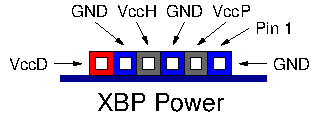
\includegraphics[scale=1]{figures/xbp_power}
    \caption{XBP Power Connector as Viewed from Front of PCB}\label{fig:power}
  \end{center}
\vspace{-1ex}
\end{figure}

\subsection{Powering the XBD}\label{sec:vccd}
Power for the XBD can be provided through the power connector's $\mathrm{V_{CC}D}$ pin.
Optionally, $\mathrm{V_{CC}D}$ can be generated on the XBP from the 5\,V $\mathrm{V_{CC}P}$.
If this is desired, please populate \textbf{IC1} with an LDO voltage regulator in a 
SOT-89-3 package. An example is the Microchip MCP1702T-3302E/MB 3.3\,V regulator.
When using such a voltage
regulator please make sure hat $\mathrm{V_{CC}D}$ pin on the power connector 
(see Fig\,\ref{fig:power}) is not connected to any power source.



\subsubsection{Using XBDs with V$_{CC} = 3.3$\,V}
If your XBD uses a V$_{CC} = 3.3$\,V and has a LaunchPad connector, you can plug it 
directly on top of the XBP. 
Otherwise you can use the XBD connector on the back of the XBP (see Fig.~\ref{fig:xbd}).
In either case, please check Chapter~\ref{sec:xbd} of this guide for details
on particular XBDs. 
When using a 3.3\,V XBD, voltage level shifting is not required. 
You can close solder jumpers \textbf{SJ1}, \textbf{SJ2}, and \textbf{SJ3}. Then
the FETs \textbf{Q3} through \textbf{Q8} and the resistors \textbf{R8} through \textbf{R11} 
should \emph{not} be populated. 

\begin{figure}[ht]
  \begin{center}
    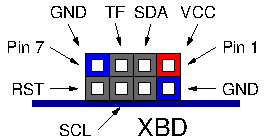
\includegraphics[scale=1]{figures/xbd_connector}
    \caption{XBD Connector as Viewed from Back of PCB}\label{fig:xbd}
  \end{center}
\vspace{-1ex}
\end{figure}

\subsubsection{Using XBDs with V$_{CC} \not= 3.3$\,V}
Such XBDs can only be connected through the XBD connector on the back (Fig~\ref{fig:xbd}).
The FETs \textbf{Q3} through \textbf{Q8} and the resistors \textbf{R8}  through \textbf{R11}
 have to be populated.
Please make sure that solder jumpers \textbf{SJ1}, \textbf{SJ2}, and \textbf{SJ3} 
are \emph{open}. $\mathrm{V_{CC}D}$ can be higher or lower than 3.3\,V.

\section{I$^2$C Pull-Up Resistors}\label{sec:i2cr}
The XBP can provide the pull-up resistors for I$^2$C. These are needed only once on an 
I$^2$C bus. We suggest that you populate \textbf{R3} and \textbf{R4} using 
10\,kOhm resistors (size: 0604) on the first XBP (XBP0).

\section{Usage without XBH}\label{sec:noXBH}
The XBP can be used also without an XBH as an experimenter's board for the INA225 
current-shunt monitor. The XBH requires $\mathrm{V_{CC}P}$ of 5\,V to be supplied
through its power connector (see Fig.~\ref{fig:power}. The power for the device 
under test can be supplied as described in section~\ref{sec:vccd}. The amplified
voltage drop over the shunt can be measured by through the SMA connector \textbf{X1}.
The gain of the amplifier can be set through jumper JP5. The jumper settings required
for the different gains are printed on the circuit board. The device under test will
get its power from the XBD connector (see Fig.~\ref{fig:xbd}). Only pins 1 and 2,
V$_{CC}$ and GND respectively, have to be used.


% -----------------------------------------------------------------------------
\chapter{XXBX Devices under Test (XBD)}\label{sec:xbd}
% -----------------------------------------------------------------------------

\section{Texas Instruments LaunchPads}

\subsection{TI Stellaris\textregistered~LM4F120 LaunchPad}

Neither the Debug, nor the Device USB should be connected for power measurements.
The \emph{+3.3V} line on pin J1.1 of the boosterpack connector is connected 
directly to the In-Circuit Debugger. Therefore, it is recommended to select on the
XBP to power the XBD via the external XBD connector and not via the boosterpack
connector. On the TI Stellaris Launchpad, the VDD jumper has to be pulled and the
external 3.3V has to be supplied to the right pin. The green power LED on the
Launchpad lights up when the 3.3V are supplied to the left (wrong) pin. 
The \emph{PWR Select} switch can be in any position and won't affect the 
measurements.

\subsection{TI Tiva\texttrademark~C Series TM4C123G LaunchPad}

The circuit connections are the same as on the TI Stellaris LaunchPad. Please follow
those instructions. Supply voltage is 3.3V with a maximum current of 300\,mA.

\subsection{TI MSP430F5529 LaunchPad\texttrademark}

For precise current measurements remove all jumpers from the isolation jumper block 
with the exception of the ground (GND) jumper. 

\subsection{TI MSP430FR6989 LaunchPad\texttrademark}

For precise current measurements remove all jumpers from the isolation jumper block 
with the exception of the ground (GND) jumper. Supply voltage is 3.3V with a maximum 
current of 2.7\,mA not including LEDs or external circuitry.

\section{ST Microelectronics NUCLEO Boards}


% -----------------------------------------------------------------------------
\chapter{XBP Assembly}
This chapter shows the assembly of the XBP. Please follow it step by step. 

\section{Indicator LEDs}
The first thing to assemble are the LEDs \textbf{LED1} for ``Power'' and 
\textbf{LED2} ``Activity'' and the associated resistors \textbf{R5} and
\textbf{R6}. The cathode of the LEDs is pointing toward the bottom of the
board. The orientation of the diode is indicated on the bottom of the LED 
with a triangle pointing toward the cathode. 
Then solder on the power connector \textbf{JP4}.

\paragraph{Test:} Test the
LEDs by applying GND to any GND pin on the power connector and touching the side 
of the resistors that does not point toward the LEDs with a wire connected to a 
3.3\,V power supply. The
``Power'' LED should light up dimly and the ``Activity'' LED should light up brightly.

\begin{figure}[ht]
  \begin{center}
    \includegraphics[scale=1]{figures/assembly-led}
    \caption{Location of LEDs, R5 and R6 on the top of the PCB}
  \end{center}
\end{figure}

\begin{cergbox}{Note: XBP without XBH}
    When using the XBP without XBH, you don't have to assemble the 
    ``Activity'' LED \textbf{LED2} or \textbf{R6} as they won't be used.
    Also skip the steps for mounting \textbf{Q1}, \textbf{Q2}, \textbf{R7},
    \textbf{R12}, and \textbf{R13}.
\end{cergbox}

\noindent Next solder the circuitry to drive the ``Activity'' LED which is located
on the bottom of the PCB. Start with the FETs \textbf{Q1} and \textbf{Q2}
and continue with \textbf{R7}, \textbf{R12}, and \textbf{R13}.

\begin{figure}[ht]
  \begin{center}
    \includegraphics[scale=1]{figures/assembly-led}
    \caption{Location of LED circuit: Q1, Q2, R7, R12, and R13 on the bottom of the PCB}
  \end{center}
\end{figure}

\section{Current-Shunt Monitor}
First solder the CSM \textbf{U1}. 
An arrow on the PCB indicates the location of pin 1. Pin 1 on the device 
is marked by a dot. Make sure that there are no solder bridges between the
pins. Then solder the current shunt in either the \textbf{R1} or the
\textbf{R2} location. If the shunt fits into the \textbf{R1} location, use it.
Next, solder the capacitors \textbf{C1} and \textbf{C3}.

\begin{cergbox}{Note: Generate $V_{CC}D$ on the XBP}
Only if you want to have the XBP generate $V_{CC}D$ for the XBP, solder \textbf{IC1}.
\end{cergbox}

\noindent Next, solder \textbf{C2}.

\paragraph{Test:} Apply 5\,V to $V_{CC}P$ on the power connector. The ``Power''
LED should light up brightly. The current consumption should not exceed 
10\,mA. If you mounted \textbf{IC1}, check with a Voltmeter that the top side
of \textbf{R1} has the desired voltage.

\begin{figure}[ht]
  \begin{center}
    \includegraphics[scale=1]{figures/assembly-led}
    \caption{Location of the CSM circuit: U1, IC1, R1, R2, C1, C2, and C3 on the top of the PCB}
  \end{center}
\end{figure}

\section{I$^2$C Pull-Up Resistors and Level Shifting}

If you want the XBP to pull-up the I$^2$C bus solder \textbf{R3} and \textbf{R4}
as discussed in section~\ref{sec:i2cr}. 

If you want to use an XBD whose $V_{CC}D \ne 3.3\,\mathrm{V}$ solder first the
FETs \textbf{Q3}, \textbf{Q4}, \textbf{Q5}, \textbf{Q6}, \textbf{Q7}, and \textbf{Q8}
followed by the resistors \textbf{R8}, \textbf{R9}, \textbf{R10}, and \textbf{R11}.

\begin{figure}[ht]
  \begin{center}
    \includegraphics[scale=1]{figures/assembly-led}
    \caption{Location of the I$^2$C pull-up: R3, R4 and level shifter: Q3--Q8 and R8--R11 on the bottom of the PCB}
  \end{center}
\end{figure}

\begin{cergbox}{Note: XBP without XBH}
    When using the XBP without XBH, you can ignore this section. 
\end{cergbox}

\section{Through-Hole Components}

First, solder the connections to the XBD (pin header) so that the pins are pointing
to the top. Then, from the bottom of the board put in the connectors for the XBH
and solder them from the top. The last connector is \textbf{JP5} which you only
have to mount if you plan on connecting an external XBD. 

\begin{cergbox}{Note: XBP without XBH}
    When using the XBP without XBH, you don't have to mount the
    launchpad connectors. Instead of mounting a complete XBD connector
    on \textbf{J2} a simple 2-pin connector on pins 1 and 2 of \textbf{J2}
    will be sufficient. Solder the gain select \textbf{JP5} and the 
    SMA connector \textbf{X1}. 
\end{cergbox}

\paragraph{Test:} bla 
% -----------------------------------------------------------------------------

\begin{appendix}
\chapter{XBP Connections}

\begin{figure}[ht]
  \begin{center}
    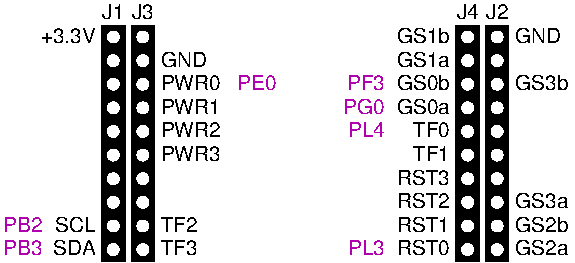
\includegraphics[scale=1]{figures/xbp-xbh}
    \caption{Boosterpack Connector XBH as Viewed from Top of PCB}
  \end{center}
\end{figure}

\begin{figure}[ht]
  \begin{center}
    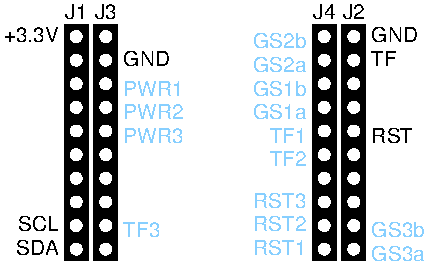
\includegraphics[scale=1]{figures/xbp-xbd}
    \caption{Boosterpack Connector XBD as Viewed from Top of PCB}
  \end{center}
\end{figure}
\begin{table}[ht]
  \begin{center}
    \caption{Pin Configuration of Boosterpack Connector for XBH}
    \begin{tabular}{rlll}
      Connector & Pin  & Net         & Comment  \\ \hline
       J1 & 1  & +3V3      & Supply Voltage $\mathrm{V_{CC}H}$ from XBH for I$^2$C pull-up resistors on XBP0 \\
       J1 & 9  & SCL       & I$^2$C Serial Clock  \\
       J1 & 10 & SDA       & I$^2$C Serial Data \\ 
       J3 & 21 & +5V       & Supply Voltage $\mathrm{V_{CC}P}$ from XBH for the XBP0 \\ \hline

       J3 & 23 & PWR0      & Analog signal of current consumption of XBD0 from XBP0\\
       J4 & 37/38 & GS0a/GS0b & Gain select for current monitor of XBD0 on XBP0\\
       J4 & 36 & TF0       & Timer Flag from XBD0 \\
       J4 & 31 & RST0      & Reset of XBD0 \\ \hline

       J3 & 24 & PWR1      & Analog signal of current consumption of XBD1 from XBP1 \\
       J4 & 39/40 & GS1a/GS1b & Gain select for current monitor of XBD1 on XBP1\\
       J4 & 35 & TF1       & Timer Flag from XBD1 \\
       J4 & 32 & RST1      & Reset of XBD1 \\ \hline

       J3 & 25 & PWR2      & Analog signal of current consumption of XBD2 from XBP2 \\
       J2 & 11/12 & GS2a/GS2b & Gain select for current monitor of XBD2 on XBP2\\
       J3 & 29 & TF2       & Timer Flag from XBD2 \\
       J4 & 33 & RST2      & Reset of XBD2 \\ \hline

       J3 & 26 & PWR3      & Analog signal of current consumption of XBD3 from XBP3 \\
       J2 & 13/18 & GS3a/GS3b & Gain select for current monitor of XBD3 on XBP3\\
       J3 & 30 & TF3       & Timer Flag from XBD3 \\
       J4 & 34 & RST3      & Reset of XBD3 \\ \hline

       J2 & 20 & GND       & \\
       J3 & 22 & GND       & \\ \hline
    \end{tabular}
  \end{center}
\end{table}
\begin{table}[ht]
  \begin{center}
    \caption{Pin Configuration of Boosterpack Connector for XBD}
    \begin{tabular}{rlll}
      Connector & Pin  & Net         & Comment  \\ \hline
       J1 & 1  & +3V3      & Supply Voltage, current is measured by XBP \\
       J1 & 9  & SCL       & I$^2$C Serial Clock  \\
       J1 & 10 & SDA       & I$^2$C Serial Data \\
       J2 & 16 & RST       & Reset of XBD \\ 
       J2 & 19 & TF        & Timer Flag to start/stop execution timer on XBH \\
       J2 & 20 & GND       & \\
       J3 & 22 & GND       & \\ \hline
    \end{tabular}
  \end{center}
\end{table}

\chapter{Schematic}\label{sec:schematic}

\begin{figure}[ht]
    \vspace{-1.6cm}
    \hspace{-1.2cm}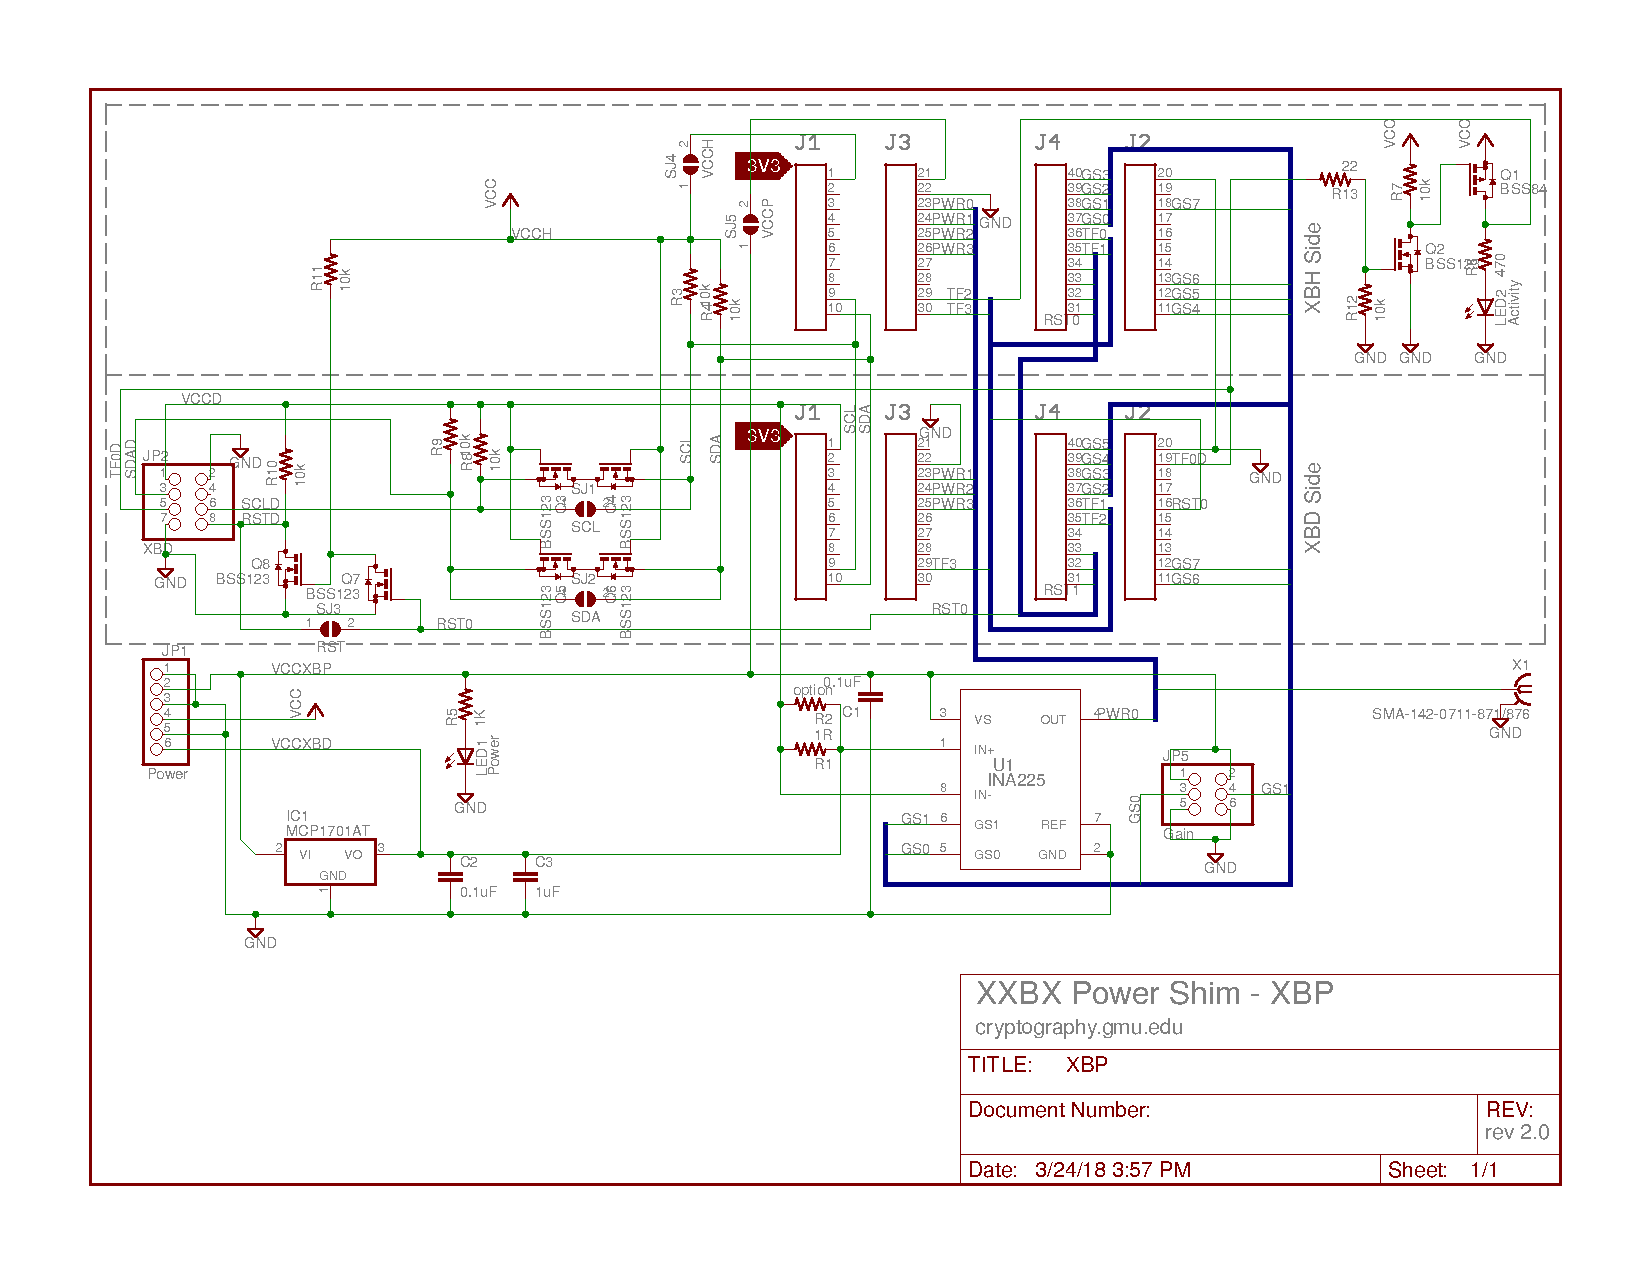
\includegraphics[scale=0.88, angle=90]{figures/XBP-schematic}
\end{figure}

\chapter{Board Layout}\label{sec:board}
\begin{figure}[ht]
  \begin{center}
    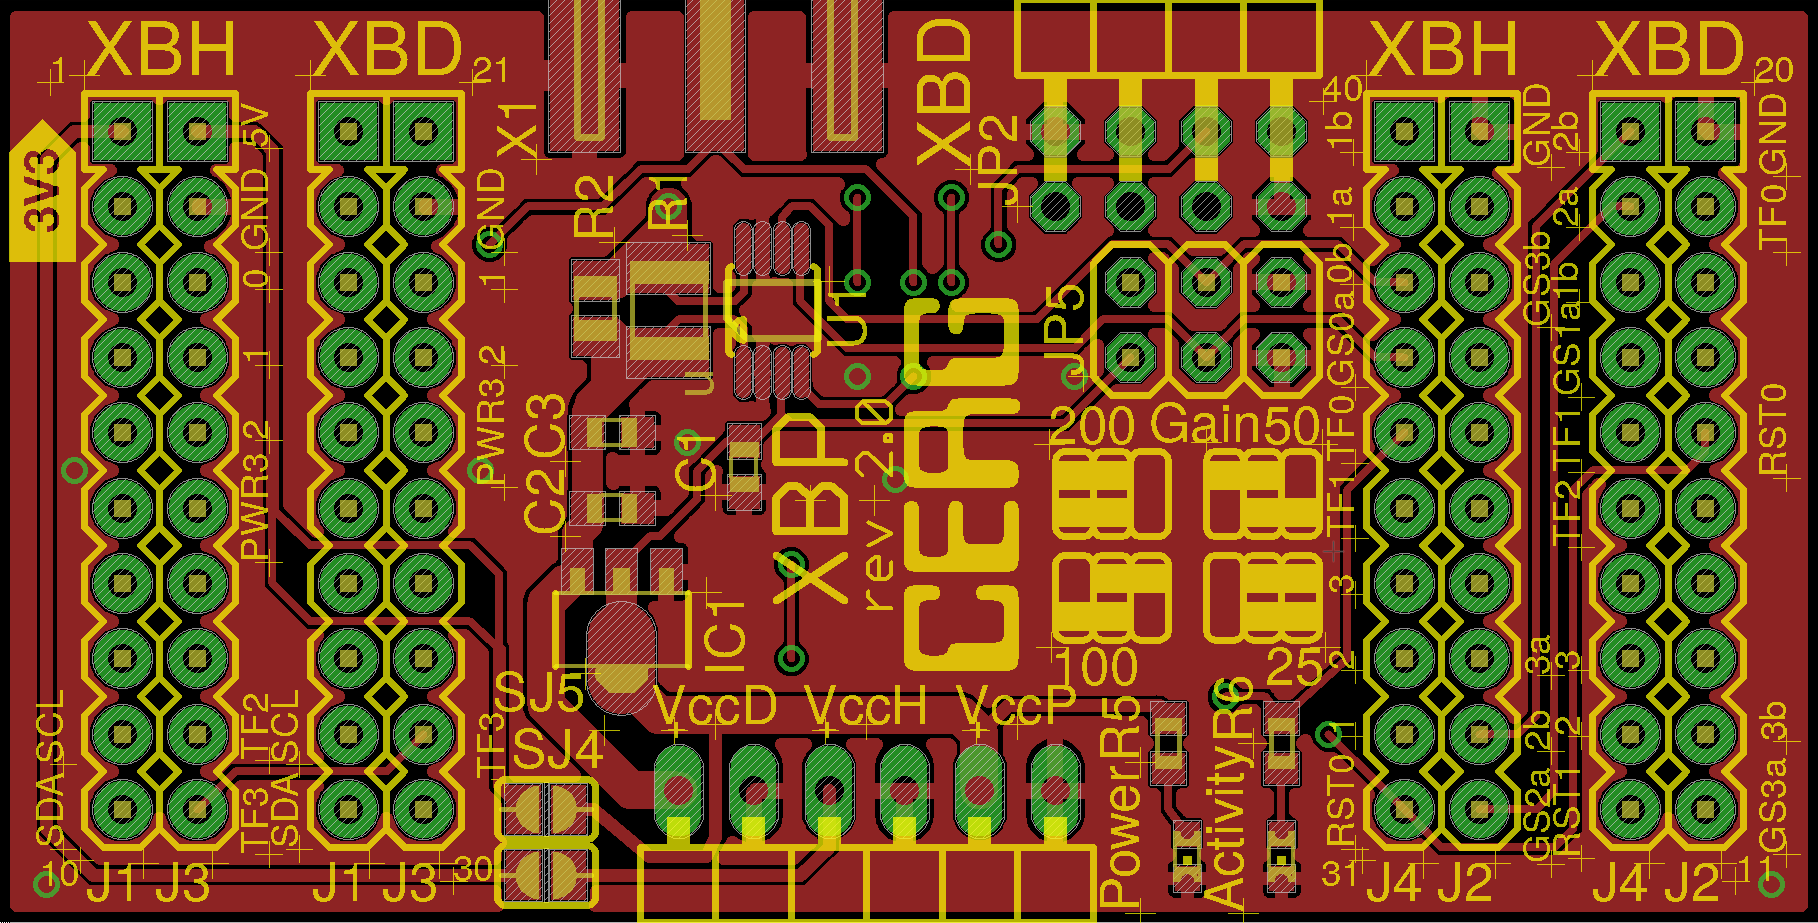
\includegraphics[scale=0.25]{figures/XBP-top}
    \caption{Top of the Circuit Board}
  \end{center}
\end{figure}

\begin{figure}[ht]
  \begin{center}
    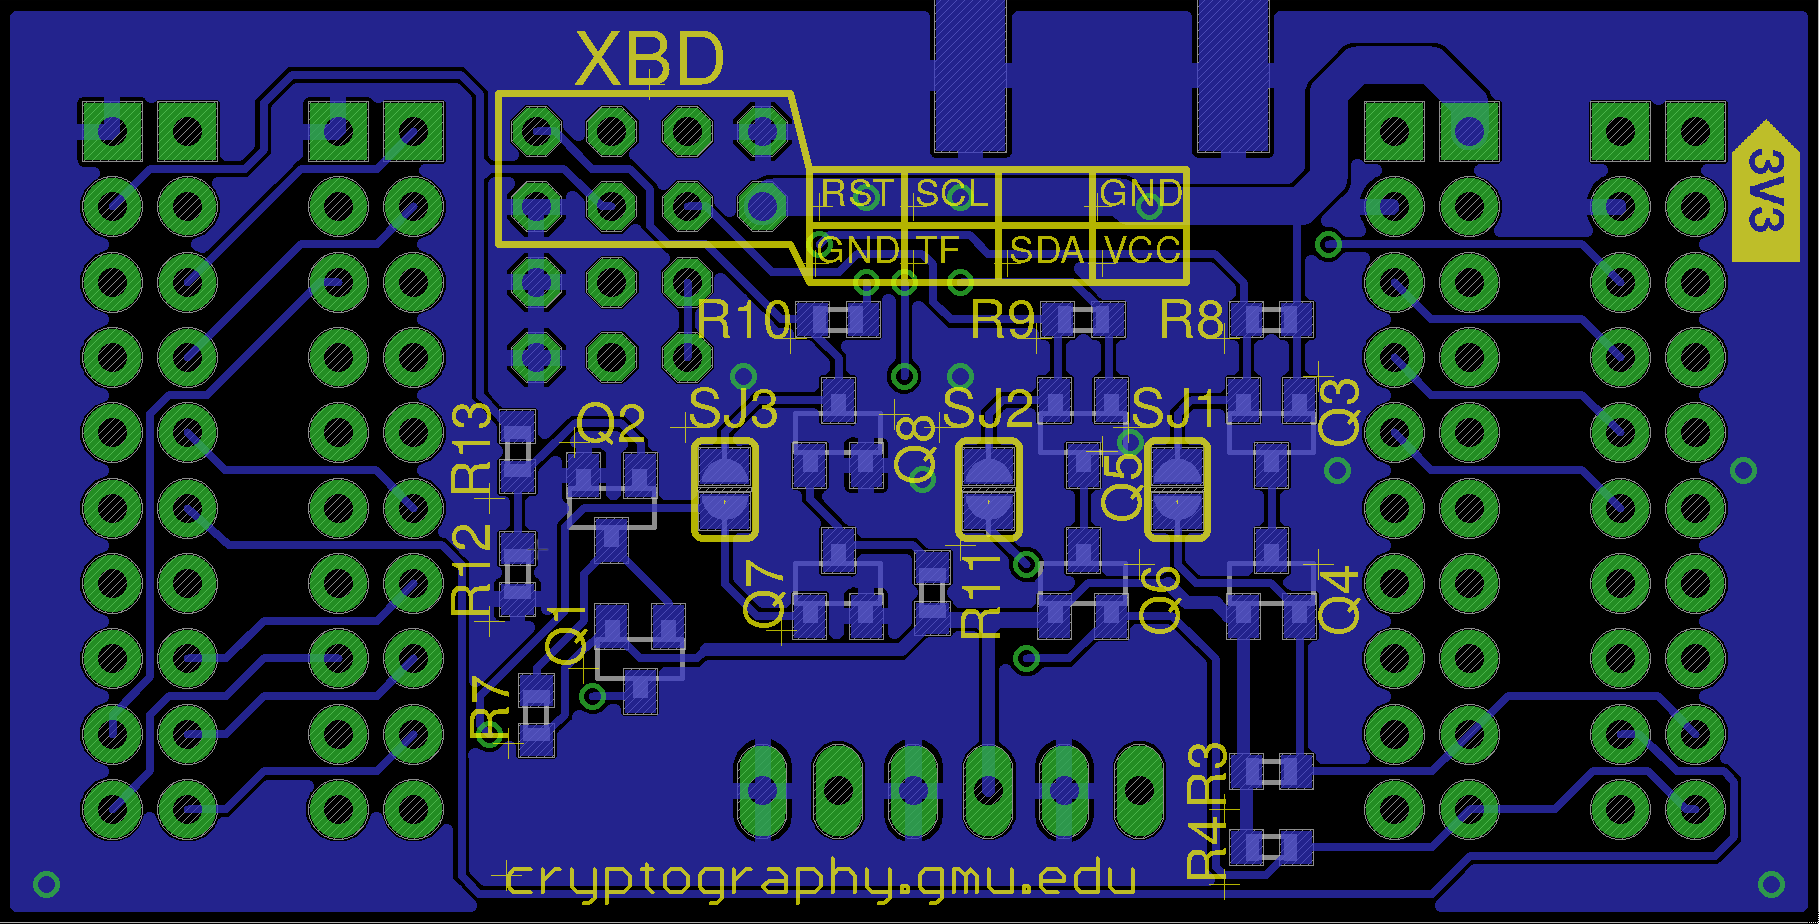
\includegraphics[scale=0.25]{figures/XBP-bottom}
    \caption{Bottom of the Circuit Board}
  \end{center}
\end{figure}
\chapter{Parts List}\label{sec:parts}

\end{appendix}


\end{document}
